\documentclass[]{article}
\usepackage{amsthm}
\usepackage{amsmath}
\usepackage{mathrsfs}
\usepackage{amssymb,amsfonts}
\usepackage[all,arc]{xy}
\usepackage{enumerate}
\usepackage{mathrsfs}
\usepackage{extarrows}
\usepackage{mathtools}
\usepackage{tikz}
\usepackage{hyperref}
\usetikzlibrary{arrows}
\usetikzlibrary{graphs}
\usetikzlibrary{graphs.standard}
\usepackage{pifont}
\newcommand{\cmark}{\ding{51}}
\newcommand{\xmark}{\ding{55}}
\def\ZZb{\mathbb{Z}_2}
\def\ZZ{\mathbb{Z}}
\def\Soc{\rm soc}
\def\FF{\mathbb F}
\def\CC{\mathbb C}
\def\RR{\mathbb R}
\def\NN{\mathbb N}
\def\CB{\mathcal B}
\def\CL{\mathcal{L}}
\def\tprod{\bigotimes}

\newcommand{\bmat}[4]{\begin{bmatrix} #1 & #2 \\ #3 & #4\end{bmatrix}}



%theoremstyle{plain} --- default
\newtheorem{thm}{Theorem}[section]
\newtheorem{cor}[thm]{Corollary}
\newtheorem{prop}[thm]{Proposition}
\newtheorem*{prop*}{Proposition}
\newtheorem{lem}[thm]{Lemma}
\newtheorem{conj}[thm]{Conjecture}
\newtheorem{quest}[thm]{Question}

\theoremstyle{definition}
\newtheorem*{defn}{Definition}
\newtheorem*{defns}{Definitions}
\newtheorem{con}[thm]{Construction}
\newtheorem*{exmp}{Example}
\newtheorem*{exmps}{Examples}
\newtheorem{notn}[thm]{Notation}
\newtheorem{notns}[thm]{Notations}
\newtheorem{addm}[thm]{Addendum}
\newtheorem{exer}[thm]{Exercise}

\theoremstyle{remark}
\newtheorem{rem}[thm]{Remark}
\newtheorem{rems}[thm]{Remarks}
\newtheorem{warn}[thm]{Warning}
\newtheorem{sch}[thm]{Scholium}




\makeatletter
\let\c@equation\c@thm
\makeatother
\numberwithin{equation}{section}

\bibliographystyle{plain}

%--------Meta Data: Fill in your info------
\title{M3/4 P55 Algebraic combinatorics}

\date{Spring 2015}

\begin{document}

\maketitle

\tableofcontents

\section*{Introduction}
	\begin{itemize}
		\item Combinatorics is a study of discrete structures.
		\item in the scope of this course we will deal with:
		\begin{itemize}
			\item Codes
				\begin{itemize}
				\item Subsets of $\ZZb^n$ where $\ZZb = \{0,1\}$
				\end{itemize}
			\item Graphs
				\begin{itemize}
				\item sets of vertices with edges connecting them. Essentailly a set with a collection of pairs. They can also be represented as adjacency matrices
				\end{itemize}
			\item Designs 
				\begin{itemize}
					\item Originated in statistical theory of experiments
					\item Collections of subsets of agiven set
				\end{itemize}
		\end{itemize}
		\item We will use tools from linear algebra to study those discrete structurs.
		\item \url{http://wwwf.imperial.ac.uk/~mwl/m3p17/}
	\end{itemize}

\subsection{Codes}
	Everyday language consists of an alphabet and words which are distinguished admissible strings of letters.\\
	\\
	For a machine language the alphabet is going to consist of:
	\begin{itemize}
		\item alphabet = $\{0,1\}$
		\item some admissible combinations of those letters (strings) e.g. $001010$, we are going to call these codewords
	\end{itemize}

	Eg. ASCII code for keyboard symbols maps each letter to 0s and 1s, 7bit words (binary strings 7 letters long)\\
	\\
	A corresponds to $01000001$\\
	B corresponds to $01000010$\\
	\\ And so on\\

	\begin{exmp}\hfill\\
	Message: Liebeck has £10000\\
	encoded into ASCII codewords:\\
	\[
	L \rightarrow 01001100
	\]
	etc.\\

	Transmitted over a digital medium.\\
	\\
	Then receiver takes the string of binary codewords and decodes it using the ASCII map, giving back the original message: “Liebeck has £1000”\\
	\\
	Suppose the bank has refused the message. Errors can occur at transceiver stage on average in 1 in 1000 bits (for example)
\\
	\\
	Different kinds of errors can occur (replace 1 with 0, lose a bit of information or cut off)
\\
	\\
	This calls for error correction schemes. Ordinary language has a lot of redundancies, i.e. words can easily be corrected \\
	\\
	E.g. \emph{Algubreic Cumbinatorocs} can easily be corrected, because there are not many similar words in the English language, and there is a set of admissible words in English, not every combination of letters is a word.\\
	\\
	Machine language should have a similar correction scheme - part of the theory of machine languages is to build in some redundancy into the language\\
	\end{exmp}

	\begin{exmp}\hfill\\
	E.g. Yes/No code:\\
	message is 1 or 0\\
	\\
	Sending just one or zero is not sufficient, because you could send a wrong digit and get the wrong answer\\

	one example of such redundant code would be to map the words the following way:
\\	
		\begin{align*}
			\text{yes} &\rightarrow 111\\
			\text{no} &\rightarrow 000\\
		\end{align*}
	If a single error is made, e.g. we send 011 instead of 111 we can correct it
	\end{exmp}
	This is called an error correcting code, and this code corrects 1 error\\
	\\
	Suppose we want to send messages in a larger language, consisting of more than 2 messages.\\
	\begin{exmp}
		This code will be able to send 8 messages and correct 1 error (the code contains 8 codewords)\\
		\\
		Messages: $abc$ in $\ZZb$\\
		Codewords:\\
		\begin{align*}
			&abcxyz \qquad (a,b,c \in ZZ_2) \text{and $xyz$ depend on $abc$}\\
			&x = a+b\\
			&y = b+c\\
			&z = a+c\\
		\end{align*}
		$C = \{000 000, 100 101, … , 111 000\}$\\
		Suppose we receive $011 110$:\\
		Well:\\
		\begin{align*}
			a + b &= 1 &= x\\
			b + c &= 0 &\neq y\\
			a + c &= 1 &\neq z = 0\\
		\end{align*}
		So there is an error. Where is it? Well it is in $c$ because it breaks the $y$ and $z$ checksums\\
		So the corrected codeword is $010 110$\\
		\\
		Claim:\\
		This code can correct 1 error\\
		\begin{table}[h]
		\begin{tabular}{lllllll}
		Error in: & \multicolumn{1}{l|}{a} & \multicolumn{1}{l|}{b} & \multicolumn{1}{l|}{c} & \multicolumn{1}{l|}{x} & \multicolumn{1}{l|}{y} & \multicolumn{1}{l|}{z} \\ \hline
		$x=a+b$   & \xmark & \xmark & \cmark & \xmark & \cmark & \cmark  \\
		$y=a+c$   & \cmark & \xmark & \xmark & \cmark & \xmark & \cmark  \\
		$z=a+c$   & \xmark & \cmark & \xmark & \xmark & \cmark & \cmark 
		\end{tabular}
		\end{table}
		So pattern of \cmark and \xmark determines the eror	
	\end{exmp}
	The aim of coding theory: Find codes $C $ s.t:\\
	\begin{itemize}
		\item $C$ has lots of codewords
		\item $C$ corrects “enough” errors
		\item We don’t want the codewords to be “too long”
	\end{itemize}
\subsection{Graphs}
	A \emph{graph} is a pair $(V, E)$ where $V$ is the set of \emph{vertices} and $E$ is a collection of pairs: $\{\{x,y\}: x,y \in V\}$ called \emph{edges}\\
	\\
	E.g. $V = \{1,2,3,4\}, \qquad E = \{\{1,2\}, \{1,3\}, \{2,4\}, \{2,3\}\}$\\

	\begin{tikzpicture}
		\graph [simple] {
		subgraph K_n [n=4, clockwise];
		1 -!- 4;
		3 -!- 4;
		};
	\end{tikzpicture}

	We will study a special type of graphs that can be expressed as codes and lend themselves well to algebraic methods\\
	\begin{defn}
	For a \emph{vertex} $x$, call the other vertices connected to $x$ by an \emph{edge} \emph{``neighbours''}
	\end{defn}

	\begin{defn}
	We call the graph $\Gamma$ \emph{regular} if every vertex has the same number of neighbours, say $K$. This number $K$ is called the \emph{valency} of the graph
	\end{defn}
	E.g. any polygon is a regular graph with a valency = 2\\
	\\
	\begin{tikzpicture}
		\graph [simple] {
			subgraph C_n [n=4, clockwise];
		};
	\end{tikzpicture}
	\begin{tikzpicture}
		\graph [simple] {
			subgraph C_n [n=3, clockwise];
		};
	\end{tikzpicture}
	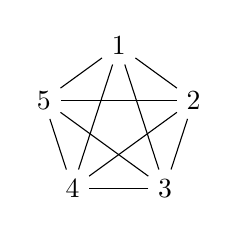
\begin{tikzpicture}
		\graph [simple] {
			subgraph K_n [n=5, clockwise];
		};
	\end{tikzpicture}

	\begin{defn}
		
A graph $\Gamma$ is \emph{strongly regular} if:
		\begin{enumerate}
		\item $\Gamma$ is regular, valency K
		\item Any pair of joined vertices has the same number a of common neighbours
		\item Any pair of non-joined vertices has the same number b of common neighbours
		\end{enumerate}
	\end{defn}

	\emph{Petersen graph} is a strongly regular graph of valency 3\\

	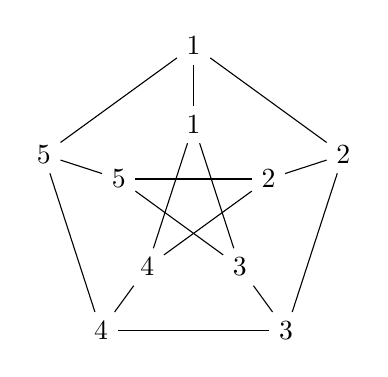
\begin{tikzpicture}
	  \graph [clockwise] {
	     subgraph C_n [n=5,name=A, radius=2cm]; 
	     subgraph I_n [n=5,name=B, radius=1cm];
	     \foreach \i [evaluate={\j=int(mod(\i+2,5)+1);}] in {1,...,5}{
	        A \i -- B \i;
	        B \i -- B \j;
	     }
	  };
	\end{tikzpicture}
	\begin{thm}[Kuratowski, 1930]\hfill\\
	A graph $G$ is planar iff $G$ does not contain a subdivision of $K_5$ or $K_{3,3}$
	\end{thm}
	\begin{proof}\hfill\\
	A Kuratowski subgraph of $G$ is a subgraph of $G$ that is a subdivision of $K_5$ or $K_{3,3}$ . A minimal nonplanar graph is a nonplanar graph such that every proper subgraph is planar.
	\end{proof}

	\begin{thm}[Friendship Theorem, Erdös, Remyi]\hfill\\
	In a community where any two people have exactly one common acquaintance, there is someone who knows everyone.
	\end{thm}
	This can be described as a graph:\\
	\\
	Vertices are the people and we join the people with edges representing the “know each other” relation\\
	\\
	The condition from the theorem is that they have one shared acquaintance, i.e. any two vertices have exactly one common neighbour\\
	\\
	We want to show that there exists a vertex that is connected to all of the other vertices in the graph\\
	\\
	\begin{tikzpicture}
		\graph [simple] {
			subgraph C_n [n=4, clockwise] -> 5;
			1 -!- 4;
			2 -!- 3;
		};
		
	\end{tikzpicture}
	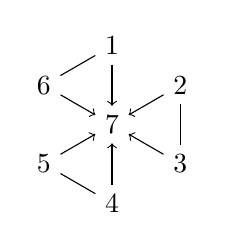
\begin{tikzpicture}
		\graph [simple] {
			subgraph C_n [n=6, clockwise] -> 7;
			1 -!- 2;
			3 -!- 4;
			5 -!- 6;
		};
	\end{tikzpicture}
	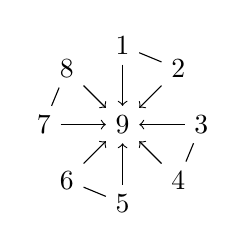
\begin{tikzpicture}
		\graph [simple] {
			subgraph C_n [n=8, clockwise] -> 9;
			1 -!- 8;
			2 -!- 3;
			4 -!- 5;
			6 -!- 7;
		};
	\end{tikzpicture}
	\\
	All the known proofs use linear algebra - matrix representations of graphs become incredibly useful/powerful\\
\subsection{Designs}
	Used in statistics and experimental design.\\
	\\
	Suppose we have v varieties of a product (say chocolate) to be tested by concumers.\\
	We want:\\
	\begin{enumerate}
		\item each consumer to test $k$ varieties
		\item each variety tested by some no. $r$ of consumers
	\end{enumerate}

	\begin{exmp}\hfill\\
		Eg. $v =9, k = 4, r =3$\\
		No of consumers must be $b = \frac{vr}{k} = 6$\\
		\\
		consumers $c_1, …, c_6$ testing:\\
		\begin{table}[h]
			\begin{tabular}{llllll}
			$c_1$  & $c_2$  & $c_3$  & $c_4$  & $c_5$  & $c_6$ \\
			$1234$ & $5678$ & $1357$ & $2468$ & $1247$ & $3568$ \\
			\end{tabular}
		\end{table}
	\end{exmp}
	\begin{defn}\hfill\\
	Let $X$ be a set, $v = |X|$ and let $\mathscr{B}$ be a collection of subsets of $X$.\\
	Call $(X, \mathscr{B})$ (or just $\mathscr{B}$) a \emph{design} if:\\
	\begin{enumerate}
		\item every set in $\mathscr{B}$ has size $k$
		\item every element of $X$ lies in $r$ subsets of $\mathscr{B}$
	\end{enumerate}
	\end{defn}
	The subsets in $\mathscr{B}$ are called the \emph{blocks} of design.\\
	Pareamters are $(v,k,r)$\\
	Example above is $(8,4,3)$\\
	\\
	Interesting condition: each pair of varieties is tested by the same number of consumers.\\
	\\
	\begin{defn}
	A design $(X, \mathscr{B}$) is a \emph{2-design} if any two points (elements of $X$) lie in the same number of blocks.

	The larger t is, the stronger this condition is.

	For large t, nontrivial t-designs are rather rare.
	(e.g. the first nontrivial 6-design was found in 1980’s).
	\end{defn}
	Example: $(8,4,3)$ is not a 2-design\\
	\\
	In general for $t \geq 1$ say $\mathscr{B}$ is a t-design if any $t$ points lie in the same number of blocks.\\
	The larger $t$ is, the stronger this condition is.\\
	For large $t$, nontrivial t-designs are rather rare. (e.g. the first nontrivial 6-design was found in 1980’s).\\
	\\
	For $t = 2$ there is a lot of nice theory, links to coding theory \& graph theory included in the course. They also lend themselves nicely to examples:\\
	\\
	\begin{exmp}[A nice example of 2 design]\hfill\\
	(Idea: take any two points in a plane, you can draw a line through them)\\
	Replace $\RR^2$ by a finite field, for example $\ZZ_p^2$\\
	Let $p$ be a prime, recall:
\\
	\[
		\ZZ_p = \text{integers up to p-1}
	\]
	with addition and multiplication mod p (ring structure) - making it a field (group under addition $\ZZ_p\setminus\{0\}$ a group under multiplication, plus obeys distributive laws).\\

	Now let $\ZZ_p^2 = \text{vectors with coordinates in $\ZZ_p$}$\\
	Call it the \emph{affine plane} over $\ZZ_p$\\
	\\
	Define a line in $\ZZ_p^2$ to be a subset of the form  $\{a + \lambda b: \lambda \in \ZZ_p\}$
	where $(a,b)$ are fixedvectors in $\ZZ_p^2$

	Fact (exercise) any two vecros in $\ZZ_p^2$ are in a unique line
	Now define:
	\begin{align*}
		X &= \ZZ_p^2\\
		\text{Blocks}\; &= \;\text{collection of lines}
	\end{align*}
	 Then this is a 2-design with parameters: $(p^2, p, p+1)$ (convince yourself it’s not $p$) where any 2 points lie in exactly 1 block (they are tested against each other once)\\
	\end{exmp}

\section{Error correcting codes}
	Define $\ZZb = {0,1}$ with addition and multiplication modulo 2\\
	\\
	and $\ZZb^n = \{(x_1,…, x_n): x_i \in \ZZb\}$ (often we will drop brackets and commas)\\ with the usual addition and scalar multiplication of vectors.\\
	$\ZZb^n$ is vector spaces over $\ZZ_2$ with standard basis $e_1, …,e_n (e_i = 0,…1,…0)$ (1 in ith place) and dimension $n$.

	\begin{defn}
		 A code $C$ of length $n$ is a subset of $\ZZ_2^n$. The vectors in $C$ are called \emph{codewords}.
	\end{defn}
	% numbering here?
	\begin{defn}
		Distance between two vectors in $\ZZ_2^n$ is:\\
		$d(x,y) = \sum_i x_i - y_i$ (number of places where they are different)

	\end{defn}
	Claim this is a metric on $\ZZ_2^n$, (i.e. it satisfies the triangle inequality)
	\begin{prop}[Triangle inequality]\hfill\\
	$d(x,y) + d(x,z) \geq d(x,z)$
	\end{prop}
	\begin{proof}\hfill \\
	Let:\\
	\begin{align*}
		A &= \{i: x_i \neq{!=}z_i\}\\
		B &= \{i: x_i = y_i, x_i \neq{!=} z_i\}	\\
		C &= \{i: x_i \neq{!=} y_i, x_i \neq{!=} z_i\}\\
	\end{align*}
	So $C$ is the compliment of $B$ in $A$\\
	So |$A| = |B| + |C|, d(x,z) = |A|$\\
	and since $d(x,y) \geq |C|$ and $d(y,z) \geq|B|$ we get the triangle inequality
	\end{proof}

	\begin{defn}\hfill\\
	Let $C \subseteq \ZZ_2^N$ be a code\\
	The minimum distance $d(C)$ of $C$ is:\\
	\[
		d(C) = min \{ d(x,y): x,y \in C, x \neq y\}
	\]
	\end{defn}

	\subsection{Error correction}
		Let $C$ in $\ZZ_2^n$ and $e\in \NN$. 
		Suppose a codeword $c \in C$ is sent and at most $e$ errors are made.\\
		Additionally, suppose a vector $v$ is received.\\
		Then we say $C$ corrects $e$ errors if the closest codeword to $v$ is $c$.\\
		\begin{defn}\hfill\\
		$C \in \ZZ_2^n$ corrects $e$ errors if for any $c_1, c_2 \in C$ and $w \in \ZZ_2^n$:\\
		\[
			d(c_1,w) \leq e, d(c_2, w) \leq e\quad \Rightarrow \quad c_1 = c_2
		\]%check here

		Equivalent definition:\\
		\\
		For $c \in C$ define sphere $S_l(c) = {w \in \ZZ_2^n: d(c,w) \leq l}$\\
		Then $C$ corrects $e$ errors if for all $c1, c_2 \in C, \quad c_1\neq2 $:\\
		\[
			S_e(c_1) \cap S_e(c_2) \neq \emptyset
		\]

		\end{defn}
		\begin{prop}\hfill \\
		Code $C$ corrects $e$ errors $\Leftrightarrow \quad d(C) \geq 2e+1$
		\end{prop}
		\begin{proof}\hfill\\
		$(\Rightarrow)$ Excercise sheet\\
		$(\Leftarrow)$: \\
		Suppose $d(C) \geq 2e+1$\\
		Let $c_1, c_2 \in C $ and suppose $w \in \ZZ_2$ satisfies $d(c_1, w) \leq e, d(c_2,w) \leq e$\\
		\\
	 	Then by the triangle inequality\\
	 	\begin{align*}
		d(c_1,c_2) &\leq d(c_1,w) + d(c_2, w)\\
		d(c_1,c_2) &\leq 2e\\
		\end{align*}
		but $d(C) \geq 2e +1$\\
		so $C$ corrects $e$ errors and $c1 = c2$\\
		\end{proof}
	\subsection{Linear codes}
		\begin{defn}\hfill\\
			A linear code is a code $C$ which is a subspace of $\ZZ_2^n$\\
		\end{defn}
		I.e:\\
		\begin{enumerate}
			\item $0 \in C$
			\item $x,y \in C \Rightarrow x+y \in C$ (subgroup group under addition)
		\end{enumerate}
		Basic construction of codes using matrices:
		\begin{prop}
			Let $A$ be an $m \times n$ matrix over $\ZZ_2$\\
			then $C = {x \in \ZZ_2^n\quad:\quad Ax = 0}
$ is a linear code and $dim C = n - rank(A)
$
		\end{prop}
		E.g:\\
		\begin{align*}
			C_3 &= \left\{abcxyz \in \ZZ_2^6\quad :\quad x = a +b, y + b+c, z = a +c \right\}\\
	       &= \left\{ x \in \ZZ_2^6\quad :\quad \left(\begin{smallmatrix}
	       			1&1&0&1&0&0\\
	       			0&1&1&0&1&0\\
	       			1&0&1&0&0&1\\
	       		\end{smallmatrix}\right) x = 0\right\}
		\end{align*}
		is a linear code of dimension 3 with basis $100101,\ 010110,\ 001011$

		\begin{prop}\hfill\\
			If $C$ is a linear code of dimension $k$, then the number of codewords :$|C| = 2^k$
		\end{prop}
		\begin{proof}\hfill''
		 Let $c_1, ..., c_k$ be a basis of $C$\\
		 \\
		Every $c \in C$ is a unique linear combination of the basis elements:\\
			\[
			c = \lambda_1 c_1 + ... + \lambda_k c_k \qquad \lambda_i \in \ZZ_2
			\]

		There are 2 choices for each $\lambda_i$, giving $2^k$ choices for $\sum_{i=0}^k\lambda_i c_i$ giving $2^k$ codewords.
		\end{proof}
	\subsection{Minimum Distance}
		\begin{defn}
			For $x \in \ZZ_2^n$, the weight of $x$ is $wt(x) = \text{no of coords of x equal to 1}$
		\end{defn}
		Observe:\\
		$wt(x) = d(x, 0)$ and $wt(x+y) = d(x,y)$, as $x+1$ has a $1$ precisely at the coords where $x$ and $y$ differ\\
		\\
		\begin{prop}\hfill\\
		Let $C$ be a linear code, then minimum distance $d(C)$ between codewords is:\\
		\[
			d(C) = \text{min} \{ wt(c)\quad:\quad 0 \neq c \in C\}
		\]
		\end{prop}
		\begin{proof}\hfill\\
		Let $c \in C, c \neq 0$ have minimal weight say $wt(c) = r$\\
		As $C$ is linear, $0 \in C$, and $d(c,0) = wt(c) = r$\\
		Therefore we have found two codewords, $r$ apart\\
		So $d(C) \leq r$\\
		\\	
		Now let $x,y$ be codewords in $C x,y\quad \neq \quad 0, x\quad \neq \quad y$\\
		\\	
		Then $x+y \in C$ and so \\
		\\	
		\[
			wt(x+y)\geq r 	
		\]
		Hence $d(x,y) = wt(x+y) \geq r$ \\
		So $d(C) \geq r$ Therefore $d(C) = r$\\
		\end{proof}
		Example:
		Code $C_3 \in \ZZ_2^6$\\
		Check that min $\{wt(c) \quad:\quad 0 \neq c \in C_3\} = 3$\\
		Hence $d(C_3) = 3$ so $C_3$ corrects 1 error by prop 1.2\\
		\\

		Aims:\\
		Find linear codes $C \in \ZZ_2^n$ s.t:\\
		\begin{itemize}
		\item $dimC$ is large
		\item $d(C)$ is large
		\item length is small
		\end{itemize}

		Matrix algebra will provide us with nice tools to achieve that.
	\subsection{Check matrix}

		\begin{defn}
		Suppose \(A\) is a \(m \times n\) matrix over \(\ZZb\) and:
		\begin{equation*}
		C = \{ x \in \ZZb^n : Ax = 0\}
		\end{equation*}
		We call A a check matrix of the linear code $C$
		\end{defn}

		\begin{prop}
		Suppose the check matrix $A$ of a linear code $C$ satisfies

		\begin{enumerate}
			\item $A$ has no $z$ column
			\item $A$ has no two equal columns
		\end{enumerate}
		Then $C$ corrects 1 error.
		\end{prop}

		\begin{proof}
		Suppose false. Then $d(C) \leq 2$ by proposition 1.2.
		Hence by propsoition 1.5 $\exists 0\neq \in C$ s.t $wt(C) = 1 || 2$

		Suppose $wt(c) = 1$. Then $c = l_i \space(=0 ... 1 ...)$ and 

		$A_C = 0 \implies Al_i = 0 \ implies ith col of A = 0$ Contradiction

		Suppose $wt(c) = 2$ then $c = l_i + l_j$ so 
		$Ac = 0 \implies Al_u + Al_j = 0 \implies ith col of A = jth col of A$ contradiction
		\end{proof}

		Examples

		\begin{enumerate}
		\item 
		\[C_3 = \{
			x \in \ZZb^6 : \begin{bmatrix}
			1 & 1 & 0 & 1 & 0 & 0 \\
			0 & 1 & 1 & 0 & 0 & 0 \\
			1 & 0 & 1 & 0 & 0 & 1
			\end{bmatrix}x = 0
		\}\]
		Corrects 1 error by 1.6

		\item Suppose we want a code $C$ which corrects 1 error and has $3 \times n$ check matrix for some n. What is max dim of $C$?
		Answer:
		By 1.6 need to find largest n s.t. $\exists 3 \times n $ check matrix with distinct non zero cols (in$\ZZb^3$). Such a matrix will have as cols all non zero vectors in $\ZZb^3$ of which there a re 7, eg:

		\[
		A = \begin{bmatrix}
			1 & 1 & 1 & 0 & 1 & 0 & 0 \\
			1 & 1 & 0 & 1 & 0 & 1 & 0 \\
			1 & 0 & 1 & 1 & 0 & 0 & 1
			\end{bmatrix}
		\]

		this is a $3\times 7$ so in check matrix of code $C$ of length 7 dim 4 (by rank nullity) correcting 1 error.

		This sends 16 messages abcd using codewords abcdxyz where 
		\[
			x = a + b + c,\\
			y = a +b + d \\
			z = a + c + d
		\]
		This is called a Hamming code $\text{Ham}(3)$

		\end{enumerate}
	\subsection{Correcting an error}
		Suppose a codeword $c$ is sent and 1 error is made, so that received vector is $c'$ which is not necessarily a code. How do we correct the error?

		Well, $c' = c + l_i$ for some $i$
		So

		\begin{align*}
			Ac' &= A(c+l_i) \\
				&= A\ c + A\ l_i \\
				&= A\ l_i \\
				&= \text{$i^\text{th}$ col of $A$}
		\end{align*}

		E.g. Let $C = \text{Ham}(3)$.
		Suppose received vector is $c= (1101000)^T$.

		Then \[
			A\ c' = \left(\begin{smallmatrix}0\\1\\0\end{smallmatrix}\right) = \text{$6^\text{th}$ column of $A$}
		\]
	\subsection{Hamming Codes}

		\begin{defn}
		Let $k\geq3$ A Hamming Code Ham$(k)$ is a code fo which the check matrix has as columns all the distinct non zero vectors in $\ZZb^k$
		\end{defn}


		\begin{prop}
		\begin{enumerate}
			\item Ham$(k)$ has length $2^k-1$, dim $2^k-1 - k$
			\item Ham$(k)$ corrects 1 error
		\end{enumerate}
		\end{prop}
		\begin{proof}
			\par
			\begin{enumerate}
			\item\par
				Since there are $2^k-1$ non zero vectors in $\ZZb^k$ check matrix of Ham$(k)$ is $k\times (2^k-1)$ and rank $k$
			\item\par
				Follows from 1.6 
			\end{enumerate}
		\end{proof}

		\begin{defn}
		Let $C, C' \subseteq \ZZb^n$. Say $C$ and $C'$ are equivalent codes if there is a permutation of the coordinates sending codewords in $C$ bijectively to codewords in $C'$. (This is equivalent to permuting the columns of the checkmatrices)
		\end{defn}

		E.g all Hamming codes ham$(k)$ are equivalent.

		We want codes that correct more than one error though. Ideally we would like to have a matrix condition that corrects lots of errors - we would like to generalize definition 1.6

		\begin{prop}
		Let $d \geq 2$ and let $C$ be a code wit hcheck matrix $A$. 
		\begin{enumerate}
			\item\par Suppose every set of $d-1$ columns of $A$ is linearly independent. If that is true, then the minimum distance $d(C) \geq d$
			\item\par Suppose in addition to (1) that $\exists$ a set of $d$ columns of $A$ that are linerarly dependent. then $d(C) = d$
		\end{enumerate}
		\end{prop}

		\begin{proof}
		\begin{enumerate}
			\item\par Suppose false, and $d(C) \leq d-1$. Then $\exists 0 \neq c \in C$ with $wt(c) = r \leq d-1$. Write $c$ as a sum of standard basis vectors: 
			\[
				c = e_{i_1} + ... + e{i_r}
			\]

			So \[
				0 = Ac = Ae_{i_1} + ... + Ae{i_r} 
			\]
			\[
				= \text{col}i_1 + ... + \text{col}i_r
			\]

			This is a contradiction, since by the hypothesis of (1) any set of $r \leq d-1$ columns is linearly independent.

			\item\par 
			Suppose columns $i_1 ... i_d$ are linearly dependent, say

			\[
				\lambda_1 (\text{col})i_1 + ... \lambda_d(\text{col})i_d = 0, \lambda_i \in \ZZb
			\]

			As by (1) any $d-1$ columns are linearly independent, all of $\lambda_i = 1 \forall i$. Then 

			\[
				0 = \text{col}i_1 + ... \text{col}i_d
			\]

			\[
				= A(e{i_1} + ... e{i_d})
			\]

			Then $c = e{i_1} + .. + e{i_d} \in C$ and $wt(c) = d$
		\end{enumerate}
		\end{proof}

		E.g

			Find a linear code of length 9 dimension 2 which corrects 2 errors.
			Answer:
			Check matrix $A$ should be a $7 \times 9$ matrix (of rank 7). 
			Also need code $C = \{x \in \ZZb^9: Ax = 0\}$ to have $d(C)\geq 5$ so by 1.8 want every set of 4 columns of $A$ to be linearly independent.

			Take
			\begin{equation*}
				A = \begin{bmatrix}
					\begin{matrix}
					| & | & \\
					\end{matrix}

					\begin{matrix}
					1 & \cdots & 0 \\
					  & \ddots & \\
					0 & \cdots & 1
					\end{matrix}
					\end{bmatrix}
			\end{equation*}

			Consisting of an $7 \times 7$ identity matrix and 2 columns $c_1, c_2$

			Need:
			\begin{enumerate}
				\item $wt(c_1)\geq 4, wt(c_2)\geq 4$ (otherwise $c_i$ and less than 3 columns of $I_7$ would be linearly dependent)
				\item $wt(c_1+ c_2) \geq 3$ (otherwise $c_1, c_2$ and $\leq 2$ columns of $I_7$ would be linearly dependent)	
			\end{enumerate}
			so take 

			\begin{equation*}
				A = \begin{bmatrix}
					1 & 0 \\
					1 & 0 \\
					1 & 0 \\
					1 & 1 & I_7 \\
					0 & 1 \\
					0 & 1 \\
					0 & 1 

					\end{bmatrix}
			\end{equation*}

			This defines the code
			\begin{align*}
				C &= \{ a b a a a (a +b)  b b b \qquad: \qquad a,b \in \ZZb \} \\
				  &= \{0^9, 101111000, 0100001111, 111110111\}
			\end{align*}
	\subsection{Hamming bounds}

		Suppose a code $C$ has length $n$ and corrects $e$ errors. How big can $|C|$ be?\\

		Recall: 
		\begin{align*}
			\text{for} v &\in \ZZb^n \\
				S_2(v) &= \{x \in \ZZb^n: d(x,v)\leq e\}
		\end{align*}

		\begin{prop}[1.9]
			$|S_e(v)| = $ sum of binomial coefficients %write this properly
		\end{prop}

		\begin{proof}
			Let:
			\begin{align*}
				d_i &= \text{no of: } x\in \ZZb^n \\
					&\text{s.t } d(v,x) = i
			\end{align*}
			Then:
			\[ |S_e(v)| = d_i + d_1 + ... + d+e\]
			The vectors at distance $i$ from $v$ are those vector differeing form $v$ in $i$ cooridinates of which there are: ${n \choose i}$ so $d_i = {n \choose i}$
		\end{proof}

		\begin{thm}[1.10, Hamming Bound]
			Let $C$ be a code of length $n$, correcting $e$ errors. \newline
			Then \[ |C| \leq \frac{2^n}{1 + n + {n \choose 2} + ... + {n \choose e}}\]
		\end{thm}

		\begin{proof}
			As $C$ corrects $e$ errors, the sphere $S_e(c)$ for $c \in C$ are all disjoint. Hence: \newline
			\begin{align*}
				| \bigcup_{c\in C} S_e(c)| &= |C| | S_e(c)| \\
											&= |C| (1 + n + .. + {n \choose e}) 
			\end{align*}

			Since $\bigcup_{c \in c} S_e(c) \subseteq \ZZb^n$, this gives \newline
			$|C| (1 + n + ... + {n \choose e}) \leq 2^n$
		\end{proof}

		Eg. Let $C$ be a linear code of length 9 correcting 2 errors. What is the maximum dimension of $C$?

		Ans. By hamming bound: \newline
			$|C| \leq \frac{2^9}{1+9+{9 \choose 2}}= 2^9/46 < 2^4$
			Hense $dim(C) \leq 3$.
			We found such a $C$ of dim 2.

			is there one of dim 3?

			To find one we need a $6 \times 9$ check matrix with any 4 cols independent. \newline
			Taking \[
				A = \begin{bmatrix}
					c_1 & c_2 & c_3 \\
					| & | & | & I_6

				\end{bmatrix}
			\]

			need $c_1, c_2, c_3 \in \ZZb^6$ to satisfy: \newline

			\begin{enumerate}
				\item $wt(c_i)\geq 4 \qquad \forall i$
				\item $wt(c_i + c_j) \geq 3 \qquad \forall i\neq j$
				\item $wt(c_1 + c_2 + c+3) \geq 2$
			\end{enumerate}

			Do $\exists$ such $c_1, c_2, c_3 \in \ZZb^6$?

			Answer: No, see problem sheet 2
	\subsection{Perfect Codes}
		\begin{defn}
			A code $C \subseteq \ZZb^n$ is  \em{e-perfect} if $C$ corrects $e$ errors and \newline
			\[
			|C| = \frac{2^n}{1 + n + .. + {n \choose e}}
			\]

			Equivalently, the union of all the (disjoint) spheres $S_e(c)\qquad (c\in C)$ is the whole of $\ZZb^n$.
		\end{defn}

		1-perfect codes

		\begin{prop}[1.11]
			Let $C \subseteq \ZZb^n$. Then \newline
			\[
				|C| = \frac{2^n}{1+n} \iff n=2^k-1, |C| =26 2^n-k 
			\]
			for some $k$
		\end{prop}

		\begin{proof}
			
			$\Rightarrow$ \newline
			If $|C| = \frac{2^n}{1+n}$ then $1 +n = 2^k$ for some $k$ \newline
			$\Leftarrow$ Clear
		\end{proof}

		Recall that Hamming code Ham$(k)$ has length $n= 2^k-1$, dimension $n-k$ and corrects 1 error. Hence: \newline

		\begin{prop}[1.12]
			Ham$(k)$ is a 1-perfect code.
		\end{prop}

		Are there any \emph{e-perfect} codes for $e\geq2$

		E.g.\newline
		For $e=2$, we need $1+n + {n \choose 2} = 2^k$ for some integer $k$ \newline
		This is quite rare, but does happen. (ask the number theory nerds)
		\par
		Famous theorem (van-Lint, Tietraven, 1964)

		\begin{thm}
		The only \emph{e-perfect} codes are:
			\begin{enumerate}
				\item $e=1$, Ham$(k)$
				\item $n=2e+1\qquad C=\{0 ... 0, 1 ... 1\}$ of dim 1
				\item $e=3, n=23, \text{dim}C = 12$, the \em{Golay code}
			\end{enumerate}

		\end{thm}
		Miraculous arithmetic:\newline
		\[
			1 + 23 + {23 \choose 2} + {23 \choose 3} = 2^{11}
		\]

		%26.1.2015
		Hamming bound is a result for non existence of codes $C$ of length $n$, correcting $e$ errors.

		This time we will concern ourselves with an existence result


		Gilbert-Varshamov bound

		\begin{exmp}
		Let $C$ be a linear code of length $15$, correcting $2$ errors. What is the maximum dimension of $C$?

		Ans:

		Hamming bound gives

		\[
			|C| \leq \frac{2^15}{1+15 +{15 \choose 2}} = \frac{2^15}{|2|} < 2^9
		\]
		Hence $dimC \leq 8$

		More on this later.
		\end{exmp}

		\begin{thm}[G-V bound][1.12]
		Let $n,k, d$ be positive integers such that

		\[
			1 + n-1 + {n-1 \choose 2} ... + {n-1 \choose d-2} < 2^{n-k}
		\]

		Then there exists a linear code of length $n$, dimension $k$ with $d(C) \geq d$
		\end{thm}

		Eg. take $n=15, d=5$

		\[
			1 + 14 + {14 \choose 2} + {14 \choose 3}  = 1 + 14 + 91 + 364 < 512 = 2^9 = 2^{15-6}
		\]

		So G-V bound tells us that such code $C$ of dim $6$ exists.

		There may or may nto exist such codes of dim 7 or 8.
		Sadly neither Hamming bound or G-V bound give us anything about the answer to this.


		\begin{proof}
			Assume the G-V bound equation. We want to construct a check matrix $A$ such that:\tabularnewline
			\begin{enumerate}
				\item $A$ is $(n-k) \times n$ (of rank $n-k$)
				\item any $d-1$ columns of $A$ are linearly independent
			\end{enumerate}
			We construct such a matrix inductively, column by column.

			Start by choosing the first $n-k$ columns:
			\[
				\begin{bmatrix}
				e_1 ... e_{n-k}\\
				\end{bmatrix}
			\]

			(inductive step)
			Suppose we've chosen $i$ columns $c_1, ..., c_i \in \ZZb^{n-k}$ \tabularnewline
			Where $n-k \leq i \leq n-1$ s.t any $d-1$ columns from $c_1 ... c_i$ are linearly independent. \tabularnewline
			Then:
			\[
				A_i = (c_1, ... , c_i)
			\]

			is $(n-k)*i$ and satisfies (2)

			For the inductive step we need to choose a further column $c_{i+1}$ so that $A_{i+1} = (c_1, ..., c_i, c_{i+1})$ still satisfies 2

			%But since $n-k \leq i$	we can choose a column that is not in the span of the first i columns.
			How many ``bad'' vectors are there - vectors in $\ZZb^{n-k}$ which are the sum of $\leq d-2$ fo the vectors from $c_1, ... , c_i$

			There are at most $1 + i  + {i \choose 2} + {i \choose 3} ... + {i \choose d-2}$ such vectors.

			But since $i$ is at most $n-1$, this is less than $2^n-k$ by the G-V bound. So therefore there is a vector in $\ZZb^{n-k}$ that is not a sum of $\leq d-2$ of the vectors $c_1, ..., c_i$. Hence the matrix

			\[
				A_{i+1} = (c_1, ..., c_i, c_{i+1})
			\]
			satisfies property (2)

			By this inductive step we construct $A_i$ for $i = n-k, ..., n$. The matrix $A = A_n$ is the required check matrix.	
		\end{proof}
	\subsection{The Golay Code}
		This is a 3-perfect code of length $23$, dimension $12$

		To construct it we first construct the \emph{extended} Golay code $G_24$
		Start with $H = Ham(3)$, check matrix:

		\[
			\begin{bmatrix}
			1 & 1 & 1 & 0 & 1 & 0 & 0  \\
			1 & 1 & 0 & 1 & 0 & 1 & 0  \\
			1 & 0 & 1 & 1 & 0 & 0 & 1
			\end{bmatrix}
		\]

		And its reverse K, with check matrix

		\[
			\begin{bmatrix}
			0 & 0 & 1 & 0 & 1 & 1 & 1\\
			0 & 1 & 0 & 1 & 0 & 1 & 1\\
			1 & 0 & 0 & 1 & 1 & 0 & 1
			\end{bmatrix}
		\]

		Add a parity check bit (= sum of bits) to $H, K$ to get length 8 codes $H', K'$
		% list hamming H' and K' codewords here


		Note.1 $H', K'$ are linear codes of length 8 dim 4.
		Note.2 All codewords are have weight 0, 8 or 4.

		Taking the 14 codewords of weight 4 in $H'$ you'll see that you can define a collection of blocks, forming a 3-design. ($v=8$ points, $k=4$ (size of block))

		\begin{prop}[1.13]
		$H \cap K = \{0^7, 1^7\} \qquad \&  \qquad H'\cap K' = \{0^8, 1^8 \}$
		\end{prop}

		\begin{proof}
		Let $v\in H\cap K$

		\begin{align*}
			H &= \begin{pmatrix}
				1 & 1 & 1 & 0 & 1 & 0 & 0 \\
				1 & 1 & 0 & 1 & 0 & 1 & 0 \\
				1 & 0 & 1 & 1 & 0 & 0 & 1 \\
			\end{pmatrix} \\
			v \in H & \qquad \Rightarrow \qquad v = abcd, a+b+c, a+b+d, a+c+d\\
		\end{align*}
		\begin{align*}
		\text{So} \qquad v \in K \quad\Rightarrow\quad \\
			c + (a+b+c) + (a+b+d) + (a+c+d) = 0 &\quad\rightarrow\quad a +c = 0\\
			b + d + (a + b + d) + (a + c +d)= 0 &\quad\rightarrow\quad c + d = 0 \Rightarrow a = b = c = d \\
			a + d + (a + b + c) + (a + c +d)= 0 &\quad\rightarrow\quad a + b = 0 \Rightarrow v = 0^7\quad\text{or}\quad 1^7
		\end{align*}
		\end{proof}
		%Guest lecture John Britnell
		\begin{align*}
			H = Ham(3) \qquad & \qquad H' = H + \ \text{parity check}\\
			K = \text{reverse of}\; H \qquad & \qquad K' = K + \ \text{parity check}
		\end{align*}

		\begin{defn}[The exteded Golay Code $G_24$]\hfill\\
		$G_24$ consists of all vectors in $\ZZb^24$ of the form:
		\begin{align*}
		(a +x, b +x, a + b + x), \qquad&\qquad \text{where} a,b\;\in H\\
		(\xlongleftrightarrow{8}, \xlongleftrightarrow{8}, \xlongleftrightarrow{8}), \qquad&\qquad \text{and}\;x\in L\\
		\end{align*}

		\begin{enumerate}
			\item\hfill\\
			$0^24\qquad \qquad a = b = x = 0^8$
			\item\hfill\\
			$1^24\qquad \qquad a = b = 0^8 \qquad x = 1^8$
			\item\hfill\\
			$(0^8, 1^8, 0^8) a =x = 1^8 \qquad b=0^8$
			\item\hfill\\
			$(0^8, 0^8, 0^8) a = b =x = 1^8$
			\item\hfill\\
			$a = 10001110, b = 10011001, x = 01001011$
		\end{enumerate}
		\end{defn}

		\begin{prop}
		$G_24$ is a linear code of dimension 12.
		\end{prop}
		\begin{proof}
			\begin{enumerate}
				\item[Linear]\hfill\\
					$0^24 \in G_24$

				\item[Closure]\hfill\\
					Suppose $a_1, a_2, b_1, b_2 \in H\, \qquad x_1, x_2 \in K'$\\
					Then 
					\begin{align*}
						&(a_1 + x_1, b_1 + x_1, a_1 + b_1 + x_1) + (a_2 + x_2, b_2 + x_2, a_2 + b_2 + x_2) =\\
							&= (a_1 + a_2 + x_1 + x_2, b_1 + b_2 + x_1, + x_2, a_1 + a_2 + b_1 + b_2+ x_1 + x_2) \in G_24\\
							&\text{Since:} \qquad a_1, a_2, b_1, b_2 \in H\, \qquad x_1, x_2 \in K'
					\end{align*}
				\item[Dimension]\hfill\\
				Suppose: $a_1 + x_1, b_1 + x_1, a_1 + b_1 + x_1) = (a_2 + x_2, b_2 + x_2, a_2 + b_2 + x_2)$\\
				Then:\\
				\begin{align*}
					a_1 + x_1 &= a_2 + x_2\\
					b_1 + x_1 &= b_2 + x_2\\
					a_1 + b_1 + x_1 &= a_2 + b_2 + x_2\\
				\end{align*}
					Adding $x_1 = x_2$, we get $a-1 = a2$ and $b_1 = b_2$\\
					So distinct choices of $(a,b,x)$ give distinct elements of $G_24$.\\
					\begin{align*}
						\text{So:} \quad |G_24| &= \text{number of triples}\qquad (a,b,x) \qquad \qquad a,b \in H' \quad x\in K'\\
						&= |H'|^2  |K'| = 2^4 \times 2^4 \times 2^4 = 2^12
					\end{align*}
					So $dim G_24 = 12$\\
				\item[Basis]\hfill \\
					Note that $(a+x, b+x, a+b+x) = (a,0,a) + (0,b,b) + (x,x,x)$ (all of these in $G_24$\\
					So if $a_i, b_i, x_i \quad (1\leq i \leq 4)$ are bases for $H', H', K'$ respectively, then:\\
					$(a,0,a) , (0,b,b) , (x,x,x) \qquad (1\leq i \leq 4)$ is a basis for $G_24$
			\end{enumerate}
		\end{proof}
		\begin{thm}
			$G_24$ has minimum distance 8\\
		\end{thm}[1.15]
		\begin{proof}
			Needs multiple steps. \\
			For $v,w \in \ZZb^n$ define $[v,w] = \text{number of places where $v$ and $w$ are both 1}$\\
		\end{proof}
		\begin{prop}[1.16]\hfill\\
			Let $v,w \in \ZZb^n$\\
			\begin{enumerate}
				\item $wt(w) = wt(v) + wt(w) = 2[v,w]$\\
				\item If 4 divides $wt(w)$ and $wt(w)$ then 4 divides $wt(v+w)$ iff $[v,w]$ is even\\
			\end{enumerate}
		\end{prop}
		\begin{proof}
			Let $r = wt(v),\quad s = wt(w),\quad t = [v,w]$\\
			Reordering coordinates as necessary, we can write:\\
			\[
				\begin{matrix}
					& \xlongleftrightarrow{t} & \xlongleftrightarrow{r-t} & \xlongleftrightarrow{s-t}\\
				v  =& 1 ... 1  				  &1 ... 1 					  &0 ...0		    & 0 ... \\
				w  =& 1 ... 1  				  &0 ... 0 					  &1 ...1		    & 0 ... \\
				w+w=& 0 ... 0  				  &1 ... 1 					  &1 ...1		    & 0 ... \\
				\end{matrix}
			\]
			Therefore let $wt(v+w) = (r-t) + (s-t) = r +s - 2t$\\
			2) follows immediately from 1.
		\end{proof}

		\begin{prop}\hfill\\
			If $a,b,x \in \ZZb^n$ then $[a,x] + [b,x] + [a+b,x]$ is even.\\
		\end{prop}
		\begin{proof}
			Let $r = [a,x],\qquad s = [b,x]$ and let $n$ be the number of places where $a,b,x$ all have 1.\\
			Reordering coordinates we can write
				\[
					\begin{matrix}
						& \xlongleftrightarrow{n} & \xlongleftrightarrow{r-n} & \xlongleftrightarrow{s-n}\\
					x  =& 1 ... 1  				  &1 ... 1 					  &1 ...1			&1 ...1		    & 0 ...  \\
					a  =& 1 ... 1  				  &1 ... 1 					  &0 ...0			&1 ...1		    & *  \\
					b  =& 1 ... 1  				  &0 ... 0 					  &1 ...1			&1 ...1		    & *  \\
					a+b=& 0 ... 0  				  &1 ... 1 					  &1 ...1			&0 ...0		    & *  \\
					\end{matrix}
				\]
				We have $[a+b, x] = (r-n) + (s-n) = (r+s-2n)$\\
				So: $[a,x] + [b,x] + [a+b,x] = r+s + (r+s-2n) = 2(r+s-n)$ which is even
		\end{proof}

		\begin{prop}[1.18]\hfill
		If $c \in G_24$ then 4 divides $wt(c)$.
		\end{prop}

		\begin{proof}\hfill\\
			We have $c = (a+x, b+x, a+b+x)\qquad a,b \ in H', x\in K'$\\
			So: 
			\[c \underset{v}{(a,b, a+b)} \underset{+}{+} \underset{w}{(x,x,x)}\]
			Since $a,b \in H'$ and $x\in K'$ we know 5 divides $wt(a), wt(b), wt(x)$.
			So 4 divides $wt(v), wt(w)$\\
			And $[v,w] = [a,x] + [b,x] + [a+b, x]$ which is even (prop 1.17)\\
			So $wt(v+w)$ is divisible by 4 by proposition 1.16 (2)\end{proof}



\end{document}

